\section{Boundary layer}
To introduce the concept of a boundary layer, envision a uniform flow moving in
a single direction with a constant speed $U_{\infty}$. Now, imagine placing a
slender plate in this flow, aligning its long side with the direction of the
flow. This configuration is commonly referred to as a \textit{flat plate at
zero incidence.} At the surface of the plate, the \textit{no-slip condition}
must be met, meaning the flow slows down until it comes to a complete stop at
the surface. However, this deceleration doesn't occur in a linear manner; a
significant portion of the flow maintains a uniform velocity. Only in the
vicinity of the plate's surface does the flow experience a slowdown, primarily
due to frictional forces. This specific area is termed the \textit{boundary
layer} or \textit{frictional layer.} The thickness of the boundary layer,
denoted as $\delta(x)$, is influenced by various factors, with its position
from the leading edge being the most prominent one. In reality, there is no
sharp demarcation between the uniform flow and the boundary layer. Therefore,
it is often defined as the region where the flow reaches 99\% of the velocity
of the outer flow \cite{Schlichting2018}. Refer to Figure
\ref{fig:boundary_layer_flat_plate} for a visual representation of this
concept.

\begin{figure}[H] \centering
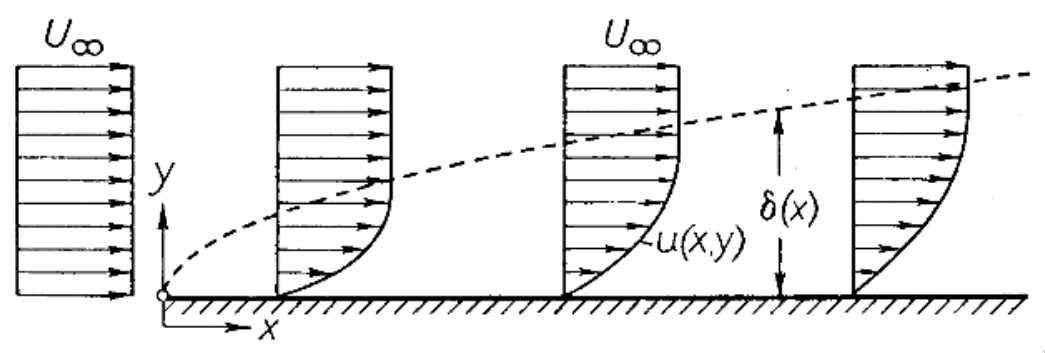
\includegraphics[width=0.5\textwidth]{boundary_layer_flat_plate}
    \caption{Laminar boundary layer of a flat plate at zero incidence
    \cite{Schlichting2018}.}
    \label{fig:boundary_layer_flat_plate}
\end{figure}

\subsubsection{Types of boundary layers}
The flow within the boundary layer can exhibit two different characteristics:
\textit{laminar} or \textit{turbulent}. In actuality, it starts as laminar at
the leading edge, then undergoes a transition to turbulence over a specific
distance, and eventually becomes fully turbulent thereafter
\cite{Schlichting2018}, this report specifically focuses on a fully turbulent
turbulence model, and as a result, the explanations of the laminar and
transitional boundary layers are not further elaborated upon.

\subsubsection{Frictional forces}
As explained earlier, the flow in the boundary layer is slowed down until it
becomes zero at the surface. This slowing down exerts a force in the flow
direction on the surface. This force, normalized by its application area, is
called \textit{shear stress} ($\tau_{w}$). To obtain a dimensionless
coefficient, which may be easily compared, the shear stress is divided by the
\textit{dynamic pressure} \cite{Schlichting2018}:

\begin{equation}
  c_{f} = \frac{\tau_{w}(x)}{\frac{1}{2}\rho U_{\infty}^{2}}
\end{equation}

\noindent Where $\rho$ is the density of the fluid and $c_{f}$ the skin friction
coefficient.


\subsection{Turbulent boundary layer}
\label{sec:turbulent_BL}
Upon closer examination of a turbulent boundary layer, one can discern two
distinct regions. The upper region constitutes a \textit{turbulent layer},
which is influenced indirectly by friction with the wall. In contrast, the
lower region is noticeably thinner compared to the overall boundary layer. This
lower region is referred to as the \textit{viscous sublayer} or \textit{viscous
wall} layer" and is directly influenced by friction. Just like the boundary
layer's broader context, there is no clear demarcation between these two
regions; instead, a smooth transition can be observed.

To analyze the cross-section of the boundary layer effectively, it is helpful
to introduce the concept of the dimensionless \textit{wall distance}, denoted
as $y^{+}$. In conjunction with this, we also consider the dimensionless
velocity, $u^{+}$. Adopting this dimensionless system facilitates the
comparison of various boundary layers from different flow conditions in a more
straightforward manner. The expression for the dimensionless velocity, $u^{+}$,
is as follows:  \cite{Schlichting2018}

\begin{equation}
  u^{+} = \frac{u}{u_{\tau}}
\end{equation}

\noindent Whereas $u$ is the flow velocity and $u_{\tau}$ the \textit{friction
velocity}. It is given by:

\begin{equation}
  u_{\tau} = \sqrt{\frac{\tau_{w}}{\rho}}
\end{equation}

\noindent As before, $\tau_{w}$ is the \textit{shear stress} and $\rho$ the
\textit{density}. The dimensionless \textit{wall distance} $y^{+}$ is given by:

\begin{equation}
  y^{+} = \frac{yu_{\tau}}{\nu}
\end{equation}

\noindent Whereas $y$ is the distance to the wall and $\nu$ is the
\textit{kinematic viscosity} of the fluid.


\subsubsection{Universal law of the wall}
Theory which describes the velocity distribution of a turbulent boundary layer
in fully developed flow\footnote{This means, the flow does not change with
increasing x.}  is know as the \textit{universal law of the wall}. It defines
the different regions as follows \cite{Schlichting2018}:

\paragraph{Viscous sublayer ($y^{+} < 5$)}
For the viscous sublayer, $u^{+}$ is given by:

\begin{equation}
  u^{+} = y^{+}
\end{equation}

\paragraph{Logarithmic overlap law ($y^{+} > 30$)}
In the fully turbulent region at the top of the boundary layer, the turbulence
stress dominates and the velocity profile varies very slowly with a logarithmic
function:

\begin{equation}
  u^{+} = \frac{1}{\kappa} ln(y^{+}) + C^{+}
  \label{eq:overlap_law}
\end{equation}

\noindent The Karman constant $\kappa$ is equal to $0.41$ and $C^{+}$ equals to
$5.0$ for smooth walls.

\paragraph{Buffer layer ($5 < y^{+} < 30$)}
The \textit{buffer layer} is located between the viscous sublayer and the
logarithmic area. It is a region where the flow transitions from one to the
other. It can not be described with such an easy equation as for the other two
regions.

If we plot the wall distance $y^{+}$ on a logarithmic scale and the velocity
$u^{+}$ on a linear scale, the different regions are obvious. Take a look at
figure \ref{fig:law_of_wall}.

\begin{figure}[H] \centering
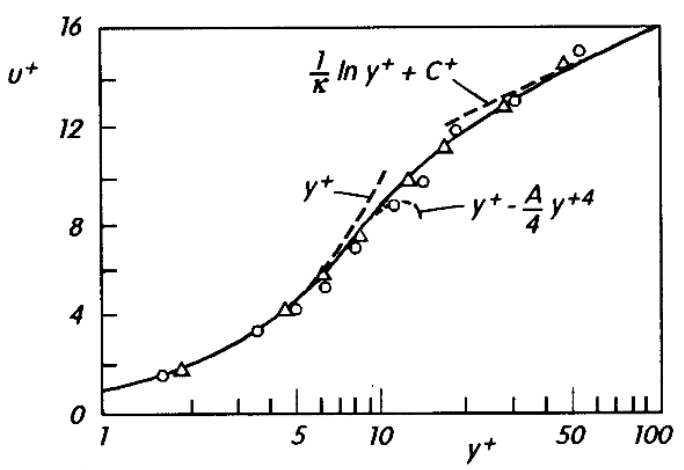
\includegraphics[width=0.45\textwidth]{law_of_wall}
    \caption{Cross-section of a fully developed turbulent boundary layer
             overlapped with measurements\cite{Schlichting2018}.}
    \label{fig:law_of_wall}
\end{figure}








\section{Reynold's Averaged Navier Stokes (RANS).}
The \textit{Navier-Stokes} equations establish the connection between the
velocity ($U$), pressure ($P$), temperature ($T$), and density ($\rho$) of a
moving fluid. These equations, represented as partial differential equations,
are typically challenging to solve analytically. Consequently, numerical
methods become necessary. The physical properties are functions of four
variables: spatial coordinates (x, y, z), and time (t). To apply numerical
methods effectively, these properties must be discretized. \cite{nasaNS}

In flows with high Reynolds numbers, various eddies have significantly
different length and time scales. Properly capturing the smallest eddies,
essentially representing turbulence, would require an extremely fine mesh and
time step, rendering it impractical. To address this challenge, simplifications
are necessary: (1) considering a steady flow instead of unsteady, and (2)
accounting for turbulence in a stochastic manner. By adopting these approaches,
a single simulation (instead of one every x milliseconds) and a coarser grid
become sufficient to achieve meaningful results.


\subsubsection{Reynolds averaging}
In 1895, Osborne Reynolds introduced a solution that would later be referred to
as \textit{Reynolds Averaged Navier-Stokes}. The fundamental concept involves
dividing the velocity (along with other resolved physical properties) into two
components: \cite{leschziner2015statistical}

\begin{equation}
    U_{i} = \bar U_{i} + u_{i}^{\prime} \qquad
    P = \bar P + p^{\prime}
\end{equation}

\noindent The subscript $i$ represents all three spatial coordinates (x, y, z).
The mean velocity, denoted as $\bar U_{i}$, remains constant, while
$u_{i}^{\prime}$ represents the fluctuating component caused by turbulence,
which remains unresolved. The same notation applies to the pressure $P$.
Substituting these expressions into the incompressible Navier-Stokes equations
results in:

\begin{equation}
    \label{eq:incomp_RANS}
    \frac{\partial \rho \bar U_{i} \bar U_{j}}{\partial x_{j}} =
    \frac{\partial \bar P}{\partial x_{i}} +
    \frac{\partial}{\partial x_{j}} \nu (\frac{\partial 
    \bar U_{i}}{\partial x_{j}} +
    \frac{\partial \bar U_{j}}{\partial x_{i}}) -
    \frac{\partial}{\partial x_{j}} \rho u_{i}^{\prime} u_{j}^{\prime}
\end{equation}

\noindent The \textit{six} independent \textit{Reynolds-stresses} are
represented by $\rho u_{i}^{\prime} u_{j}^{\prime}$. It is important to note
that the fluctuating component for pressure, $p^{\prime}$, cancels out and does
not reappear. The Reynolds stresses can be denoted using tensor notation:

\begin{equation}
    \rho \bar u_{i} \bar u_{j} = \rho
    \begin{pmatrix}
        u_{1}^{\prime 2}              & u_{1}^{\prime} u_{2}^{\prime} & 
        u_{1}^{\prime} u_{3}^{\prime} \\

        u_{2}^{\prime} u_{1}^{\prime} & u_{2}^{\prime 2}              & 
        u_{2}^{\prime} u_{3}^{\prime} \\

        u_{3}^{\prime} u_{1}^{\prime} & u_{3}^{\prime} u_{2}^{\prime} & 
        u_{3}^{\prime 2}
    \end{pmatrix}
\end{equation}

\noindent Equation \ref{eq:incomp_RANS} is complemented by the Reynolds-averaged
mass-conservation equation:

\begin{equation}
    \frac{\partial \rho \bar U_{j}}{\partial x_{j}} = 0
\end{equation}


\subsubsection{Turbulence model}
To determine the unknown Reynolds stresses, a \textit{turbulence model} is
employed. Among several approaches, the two most commonly used are \textit{Eddy
viscosity} models and \textit{Reynolds stress transport} models. The SST model
belongs to the former category, and therefore, it will be elaborated on in more
detail.

\paragraph{Eddy viscosity models}
These kind of models depend on the \textit{Boussinesq-assumption} which says
that the effect of turbulence is similar to that of an increased viscosity.
Thus, it introduces the \textit{eddy viscosity} $\mu_{t}$. After some equation
mangling one may calculate the Reynolds stresses from the eddy viscosity as
follows:

\begin{equation}
    - \rho u_{i}^{\prime} u_{j}^{\prime} =
    \nu_{t} (\frac{\partial \bar U_{i}}{\partial x_{j}} +
    \frac{\partial \bar U_{j}}{\partial x_{i}}) -
    \frac{2}{3} \delta_{ij} \rho k
    \label{eq:boussinesq}
\end{equation}

\noindent Where

\begin{align*}
    \delta_{ij} = \; &0 \qquad \text{for} \qquad i \neq j \\
    &1 \qquad \text{for} \qquad i = j
\end{align*}

\noindent and $k$ is the \textit{turbulent kinetic energy}. Thus the calculation
of the six Reynolds-stresses has reduced to calculating $\nu_{t}$ and $k$.
\cite{leschziner2015statistical}

\paragraph{Turbulent kinetic energy}
is the mean \textit{kinetic energy} per unit mass associated with eddies in
turbulent flows. It is defined as half the sum of variances of the velocity
components:

\begin{equation}
    k = \frac{1}{2} \left( 
    \overline{(u^{\prime})^2} +
    \overline{(v^{\prime})^2} +
    \overline{(w^{\prime})^2}
    \right)
\end{equation}








\section{Turbulence models}
\label{sec:turb_models}
The SST model is a mix between earlier models. It basically blends between the
$k$ - $\epsilon$ and $k$ - $\omega$ turbulence models. As such, they are
introduced first.




\subsection{$k$ - $\epsilon$ model}
This model was first introduced in 1972 and solves two transport equations.
\cite{JONES1972301} One for the turbulent kinetic energy ($k$) and one for the
dissipation rate ($\epsilon$) \footnote{The rate at which $k$ is converted into
thermal energy through viscosity}. To apply the Boussinesq-assumption, $k$ and
$\nu_t$ are needed. The first one is solved for directly and the second one is
calculated as follows:



\begin{equation}
    \label{eq:k_epsilon_nu_t}
    \nu_t = C_{\nu} \frac{\rho k^2}{\epsilon}
\end{equation}


\subsubsection{Transport equations}
\noindent The transport equations are as follows:
\begin{align}
    \label{eq:transport_k}
    \frac{\partial (\rho k)}{\partial t} + 
    \nabla \cdot (\rho U k) &=
    \nabla \cdot \left[ 
        \left( \nu + \frac{\nu_t}{\sigma_k}\right) + \nabla k 
    \right] + P - \rho \epsilon \\
%
    \label{eq:tranport_epsilon}
    \frac{\partial (\rho \epsilon)}{\partial t} + 
    \nabla \cdot (\rho U \epsilon) &=
    \nabla \cdot \left[ 
        \left( \nu + \frac{\nu_t}{\sigma_{\epsilon}}\right) + \nabla  \epsilon
    \right] + C_1 \frac{\epsilon}{k}P - 
    C_2 \rho \frac{\epsilon^2}{k}
\end{align}

\noindent Where $P$ is the production due to mean velocity shear and buoyancy.
The symbol $\nabla$ represents the spatial derivatives $\partial / \partial
x_i$ where $i$ is either in $x$, $y$ or $z$ direction. The remaining constants
have been derived from experiments and may change. Originally, they were
defined as follows:

\begin{align*}
    C_1 &= 1.55         & C_2               &= 2.0  & C_{\nu} &= 0.09\\
    \sigma_k &= 1.0     & \sigma_{\epsilon} &= 1.3
\end{align*}

\noindent The variant of this model is referred to as the
\textit{high-Reynolds-number} form. As its name implies, it performs poorly in
predicting results near walls where the Reynolds number is low. This deficiency
arises due to the blocking effects caused by the wall in the viscous sub-layer,
which reduces dissipation.


\subsubsection{Modifications for near wall flows}
The original authors proposed an extension that is better suited for flows in
the viscous sub-layer. It is called \textit{low-Reynolds-number form}. The
model is modified as follows:

\begin{align}
    \nu_t = \textcolor{red}{f_{\nu}} C_{\nu} \frac{\rho k^2}{\epsilon},  \qquad
%
    ... + C_1 \frac{\epsilon}{k}\textcolor{red}{f_1} P 
    - \textcolor{red}{f_2} C_2 \rho \frac{\epsilon^2}{k} + ..
\end{align}

\noindent Where the modifications in red are damping functions that are defined
as follows:

\begin{align}
    f_1 &= 1 \\
    f_2 &= 1 - 0.3 exp(-Re_T^2) \\
    f_{\nu} &= exp \left( \frac{-3.4}{(1 + (Re_T/50))^2}\right) \\
\end{align}

\noindent Where $Re_T$ is the turbulent Reynolds number which is:

\begin{equation}
    Re_T = \frac{\rho k^2}{\nu \epsilon} 
\end{equation}

\noindent The damping function $f_{\nu}$ tends to be 1 far from the wall
because $Re_T$ tends to be high there. Close to the wall, where $Re_T$ is low,
$f_{\nu}$ goes towards 0 and thus the effects of the eddy viscosity vanish. The
original authors did not see an improvement for $f_1$ and therefore left it at
1. The function $f_2$ is applied to the dissipation of $\epsilon$ and
consequently lowers it near the wall it.


\subsubsection{Boundary conditions}
The boundary conditions are \cite{JONES1972301}:

\begin{align*}
    k_{w}        &= 0       &\epsilon_{w} &= 0 \\
    u_{\infty} \frac{d k_{\infty}}{d x}  &= - \epsilon_{\infty}
    & u_{\infty} \frac{d k_{\infty}}{d x} &= 
    - C_2 f_2 \epsilon_{\infty}^2 / k_{\infty}
\end{align*}
\noindent Where the subscript $w$ stands for \textit{wall} and $\infty$ for the
\textit{freestream condition}.


\subsubsection{Weaknesses}
This model works well for prediction flows outside of boundary layers. Although
it has the capacity to predict the flow near the wall, inside the boundary
layer, it does so poorly. If there are \textbf{adverse pressure gradients}
and/or \textbf{shocks} present, the prediction inside the boundary layer is
even worse. \cite{cfd101_k-epsilon}




\subsection{$k$ - $\omega$ model}
Because of the shortcomings mentioned in the section before, a better
turbulence model was needed for aerodynamics and turbomachinery. This model
tried to address this by modeling the specific turbulent dissipation rate
$\omega$ instead of $\epsilon$. They are related as follows:

\begin{equation}
    \label{eq:omega_epsilon}
    \omega = \frac{\epsilon}{C_{\nu} k}
\end{equation}

\noindent where $C_{\nu} = 0.09$. Plugging this into equation
\ref{eq:k_epsilon_nu_t} leads to:

\begin{equation}
    \nu_t = \frac{\rho k}{\omega}
\end{equation}


\subsubsection{Transport equations}
The transport equations for $k$ remains the same as in equation
\ref{eq:transport_k}. But the transport equation for $\epsilon$ is replaced by
one for $\omega$. As the notation has changed slightly, the transport equation
for $k$ is also shown:

\begin{align}
    \label{eq:transport_k_omega}
    \frac{\partial (\rho k)}{\partial t} + 
    \nabla \cdot (\rho U k) &=
    \nabla \cdot \left[ 
        \left( \nu + \sigma_k \nu_t \right) + \nabla k 
    \right] + P - \rho \epsilon \\
%
    \label{eq:tranport_epsilon_omega}
    \frac{\partial (\rho \omega)}{\partial t} + 
    \nabla \cdot (\rho U \omega) &=
    \nabla \cdot \left[ 
        \left( \nu + \sigma_{\omega} \nu_t \right) + \nabla  \omega
    \right] + \frac{\gamma}{\nu_t} P - \beta \rho \omega^2
\end{align}

\noindent The constants for the Wilcox 1988 version\footnote{There a lot of
different versions for this model} are as follows: \cite{nasatmr}

\begin{align*}
    \beta       &= 3/40     & \gamma            &= 5/9\\
    \sigma_k    &= 0.5      & \sigma_{\omega}   &= 0.5
\end{align*}


\subsubsection{Boundary conditions}
The boundary conditions for the wall are equal to the $k$ - $\epsilon$ model.
As there are many different versions, it is not quite clear what the correct
values for the farfield would be. \cite{nasatmr} suggest that the ones for the
SST model should be used (see section XXX). \cite{cfd101_k-omega}

\begin{align*}
    k_{w}        &= 0           &\epsilon_{w}       &= 0 \\
\end{align*}


\subsubsection{Differences to $k$ - $\epsilon$}
While both models share similarities, the $k$ - $\omega$ model stands out by
not requiring inaccurate damping functions, making it more suitable for adverse
pressure gradients. Consequently, the $k$ - $\omega$ model significantly
outperforms the other model for flows inside boundary layers, leading to
improved predictions in the fields of aerodynamics and turbomachinery.


\subsubsection{Weaknesses}
Unfortunately, this models solution highly depends on the freestream boundary
conditions. Even small changes can lead to drastic different skin friction
coefficients. This in turn may lead to different flow separation points.
Unfortunately, it is not exactly clear where this dependence is coming from.
\cite{cfd101_k-omega}




\subsection{$k$ - $\omega$ SST model}
To recap, there is a model that works well far away from walls ($k$ -
$\epsilon$) but is not suited for flows near it. And there is a model that acts
the other way around ($k$ - $\omega$). Additionally, both models are highly
similar. Thus the Idea of the $k$ - $\omega$ SST model is to blend both models
in such a way that the $\epsilon$ formulation is used far away from walls and
the $\omega$ formulation is used near walls. Figure \ref{fig:sst_blending}
shows this concept.

\begin{figure}[H] \centering
    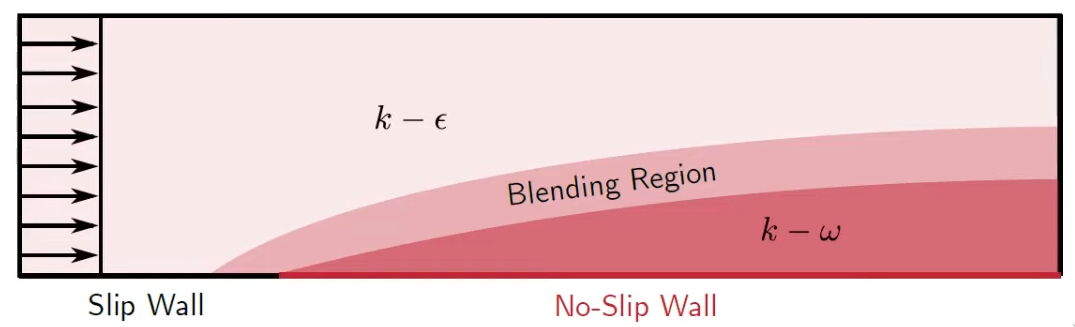
\includegraphics[width=0.7\textwidth]{sst_blending}
    \caption{Flat plate a zero incidence with SST blending between $k$ -
    $\omega$ and $k$ - $\epsilon$ where appropriate \cite{cfd101_k-omega}.}
    \label{fig:sst_blending}
\end{figure}


\subsubsection{Transport equations}
It has already been established that the transport equation of $k$ is the same
for both models (see equation \ref{eq:transport_k_omega}). When we take the
transport equation for $\epsilon$ (eq. \ref{eq:tranport_epsilon_omega}) and
substitute $\epsilon$ with equation \ref{eq:omega_epsilon}, we get:

\begin{equation}
    \frac{\partial (\rho \omega)}{\partial t} + 
    \nabla \cdot (\rho U \omega) =
    \nabla \cdot \left[ 
        \left( \nu + \frac{\nu_t}{\sigma_{\omega}}\right) + \nabla  \omega
    \right] + \frac{\gamma}{\nu_t} P_k - \beta \rho \omega^2 
    \textcolor{red}{
        + 2 \frac{\rho \sigma_{\omega 2}}{\omega} \nabla k : \nabla \omega
    }
\end{equation}

\noindent When ignoring the additional part in red\footnote{$\nabla k : \nabla
\omega$ stands for: $\frac{\partial k}{\partial x_j} \frac{\partial
\omega}{\partial x_j}$}, then it is the same equation as was used to to
transport $\omega$. When we multiply this additional term with $(1 - F_1)$, we
can blend between the two models by varying $F_1$ from 0 ($k$ - $\epsilon$) to
1 ($k$ - $\omega$). Of course, both models have different constants and they
must be blended as well:

\begin{equation}
    \phi = F_1 \phi_1 + (1 - F1) \phi_2
\end{equation}

\noindent Where subscript 1 and 2 are the respective constants from each model.
The constants for the standard Menter SST variant from 1994  are as follows:
\cite{nasatmr}

\begin{align*}
    \gamma_1 &= \frac{\beta_1}{C_{\nu}} - 
    \frac{\sigma_{\omega 1} \kappa^2}{\sqrt{C_{\nu}}}
    & \gamma_2 &= \frac{\beta_2}{C_{\nu}} - 
    \frac{\sigma_{\omega 2} \kappa^2}{\sqrt{C_{\nu}}}\\
%
    \sigma_{k 1}        &= 0.85  & \sigma_{k 2}         &= 1.0 \\
    \sigma_{\omega 1}   &= 0.5   & \sigma_{\omega 2}    &= 0.856 \\
    \beta_1             &= 0.075 & \beta_2              &= 0.0828 \\
    \kappa              &= 0.41
\end{align*}


\subsubsection{Blending function}
The blending function is computed as follows:

\begin{equation}
    \label{eq:f1}
    F_1 = tanh(arg_1^4)
\end{equation}

\noindent Where:

\begin{equation}
    \label{eq:arg1}
    arg_1 = min \left[ max \left( 
    \frac{\sqrt{k}}{\beta^{*} \omega d}, \frac{500 \nu}{d^2 \omega}
    \right), 
    \frac{4 \rho \sigma_{\omega 2} k}{CD_{k \omega} d^2}
    \right]
\end{equation}

\noindent Where $d$ is the distance to the nearest wall and $CD_{kw}$:

\begin{equation}
    \label{eq:cdkw}
    CD_{kw} = max \left( 
    2 \rho \sigma_{\omega 2} \frac{1}{\omega} \nabla k \nabla \omega, 10^{-20} 
    \right)
\end{equation}

\noindent At this point, we have got the $k$ - $\omega$ BST model.


\subsubsection{Viscosity Limiter}
 It has been found through experiments that a viscosity limiter is beneficial.
 Thus, the computation of $\nu_t$ is modified:

\begin{equation}
    \nu_t = \frac{a_1 \rho k}{max(a_1 \omega, \Omega F_2)}
\end{equation}

\noindent Where $a_1 = 0.31$, $\Omega$ is the vorticity magnitude  and $F_2$ is
a second blending function. It is computed as follows:

\begin{equation}
    F_2 = tanh(arg_2^2)
\end{equation}

\noindent Where:

\begin{equation}
    arg_2 = max \left( 2\frac{\sqrt{k}}{C_{\nu} \omega d},
    \frac{500 \nu}{d^2, \omega}\right)
\end{equation}

\noindent The closer we are to the wall, the bigger $arg_2$ is (as it depends on
this distance). The higher $arg_2$ is, the bigger $F_2$ gets. And if $F_2$ gets
bigger, the viscosity is limited more and more.


\subsubsection{Conclusion}
This model agrees better with experiments of mildly separated flows. This
is mainly due to the viscosity limiter. Hence, it is best for external
aerodynamics or simulations where separation is important. \cite{cfd101_sst}








\section{Gradient computation}
\label{sec:gradient_computation}
When optimizing, we try to minimize the objective function $o(x)$ while making
sure the constraints $c(x)$ are satisfied. The vector $x$ stands for the
\textit{design variables (DVs)}. From an outside perspective, the objective
$o(x)$ and constraints $c(x)$ are the same in the sense that we need to provide
a function value an its gradients. The distinction only happens at the
optimizer level. Thus, they are are called \textit{Functions of Interest (FoI)}
or $f(x) = \begin{bmatrix} o(x) & c(x)\end{bmatrix}^T$. Therefore, the
gradients we are after are $d f / d x$. To obtain it, we have a view different
options available: \cite{mdobook}

\begin{itemize}
    \item \textbf{Finite Differences (FD)} are the traditional approach. But
        they are inefficient as they scale with the number of DVs which can
        grow quite substantial in practical optimizations. Additionally, they
        are not that accurate as the lowest possible step is limited by machine
        precision.

    \item \textbf{Complex Step (CS)} is almost the same as FD. But the step is
        applied in the complex plane. This decouples it from the base-floating
        point number and thus allows an almost infinitely small step without
        running into machine precision problems. This means, CS is almost as
        accurate as it gets, but it is still inefficient.

    \item \textbf{Automatic/Algorithmic Differentiation (AD)} is a technique
        that is known widely as \textit{back propagation} in machine learning.
        It basically uses the chain rule in an automated and systematic manner
        to compute the total derivatives from partial derivatives based on
        basic maths operations (e.g. Additions or multiplications). There
        exists a \textit{forward} and \textit{backwards} mode. The forward mode
        computes the derivative $d f / d x$ and scales with the number of
        design variables. Thus, it is as efficient as CS or FD. But it is as
        accurate as analytic derivatives are. The backwards mode computes the
        same derivative but scales with the number of FoIs. In practical
        optimizations, the number of FoIs is usually a lot lower than the
        number of DVs. Thus the backwards mode is more efficient and highly
        desirable.

    \item \textbf{Adjoint method} is, roughly spoken, an extension to AD. The
        problem with AD for the backwards mode (which we are interested the
        most) is, that you need to store additional memory for each math
        operation. This works well in machine learning because there are no
        iterative solvers. But this is not the case here and the memory
        required is just to much. The \textit{adjoint method} bypasses this by
        replacing part, where an iterative solver is needed,  with a linear
        system which needs to be solved. So the trade is less memory footprint
        in exchange for more computing power. A trade that is well worth.
\end{itemize}




\subsection{Adjoint method}
The adjoint method\footnote{Analogous to AD, there exists also a forward mode
called \textit{direct method}} involves solving the following system (as it
scales with the number of FoIs, a system per FoI needs to be solved.):

\begin{equation}
    \psi^T = \frac{\partial f}{\partial u} \frac{\partial r}{\partial u}^{-1}
\end{equation}

\noindent Where $\psi^T$ are the adjoint vectors, $u$ are the state variables
the CFD solver solves for (e.g. pressure, velocity) and $r$ are the residuals.

Once the adjoint vectors are obtained, the total derivative can be computed as
follows:

\begin{equation}
    \frac{df}{dx} = \frac{\partial f}{\partial x} - 
    \psi^T \frac{\partial r}{\partial x}
\end{equation}


\noindent To compute the partial derivatives, any method mentioned in the
section above may be used, but is most reasonable to use AD. \cite{mdobook}



\subsection{Direct mode}
As said before, there also exists an 'opposite' mode to adjoint, it is called
\textit{direct mode}. First, we need to solve the direct vectors:

\begin{equation}
    \phi = \frac{\partial r}{\partial x} \frac{\partial r}{\partial u}^{-1}
\end{equation}

\noindent Then, we can use it to obtain the total derivatives:

\begin{equation}
    \frac{df}{dx} = \frac{\partial f}{\partial x} -
    \phi \frac{\partial f}{\partial u}
\end{equation}

\noindent This mode is less desirable as it depends on the number of DVs, but
it comes in handy for verification of the adjoint method.




\subsection{Verification}
Accurate gradients are important as they accelerate the optimization or may
even prevent it from converging at all. Thus, the partial and total derivatives
need to be verified. As the total derivatives depend on the partial ones, it
makes sense to verify them first:

\begin{enumerate}
    \item \textbf{Compare forward derivatives against FD.} As FD is not as
        accurate, it is not enough, but it is easy to implement (no
        modifications needed to the code) and shows that we are in the right
        bulk part.
    \item \textbf{Compare forward derivatives against CS.} This is absolutely
        needed to be sure. But it requires modification of the code and thus
        may introduce errors.

    \item \textbf{Dot product test} Once the forward routines are verified, we
        can apply the dot product test (see below) to verify the backwards
        routines as well.
\end{enumerate}

\noindent Once the partial derivatives are verified, we can try to solve the
adjoint system. If this is done, the total derivatives may be verified (1.)
against FD and then (2.) against CS.

\subsubsection{Dot product test}
Sometimes, it is only possible to verify the forward mode against CS, but we
are more interested in the other one. In such a situation, the
\textit{dot-product test} comes in handy as it provides a relation ship between
both modes:

\begin{equation}
    \psi_j^T \frac{\partial r}{\partial x_i} = 
    \frac{\partial f_j}{\partial u} \phi i
\end{equation}

\noindent Where $i$ and $j$ represent the column and row vectors respectively.
When both sides of the equation match to a tolerance that is slightly higher
than machine precision, we can be confident that the reverse (adjoint) method
has been implemented correctly.\cite{mdobook}




% \section{Solving RANS equations}
% ADflow has three different solvers available to solve the RANS equations:
% \textit{multigrid}, \textit{Newton Krylov} and \textit{Approximate Newton
% Krylov}. \cite{adflow_solvers} 

% Originally, only multigrid was implemented as the other two solvers need the
% partial derivatives $\partial r / \partial u$. Since they were needed for the
% adjoint implementation anyways, it was a logical next step to implement the
% Newton type solvers. This part will not go into any details, but it is
% important to state that there are two ways (in ADflow) to compute the partial
% derivatives needed: FD and AD.  


\section{Netwons method for residual equations}
Usually, the RANS equations are solved using a "dumb" algorithm such as
\textit{jacobi iteration}. It is used to solve a linear system such as:

\begin{equation}
    \label{eq:cfd_system}
    Au = b
\end{equation}

\noindent Where $u$ are the state variables (such as pressure and velocity). $b$
are the sources, an $A$ is the state matrix. As this is an iterative approach,
the solutions gets better and better the longer the algorithm runs. This means,
we need an criteria to stop. For this, we use the residual formulation:

\begin{equation}
    R(u_n) = b - Au_n 
\end{equation}
 
\noindent Where $n$ represents the value of the current iteration. Once the
residual value reaches a threshold, we stop.

When looking at the partials that are needed for the adjoint method, we realize
that we already compute the partials $\partial r / \partial u = R'(u)$. This
comes in handy as it can be used in Newtons method for the solution of equation
\ref{eq:cfd_system}:

\begin{equation}
    u_{n+1} = u_n - \frac{R(u_n)}{R'(u_n)}
\end{equation}

\noindent Newtons method does converge faster than the before mentioned "dumb"
approaches. But it is usually not implemented as the effort to obtain $R'(u)$
is not considered worth the profit. But we are interested in gradient
computation for optimizations and thus need the partials anyways. So it makes
sense to use Newtons method "free of charge". This is exactly what ADflow does
with its \textit{Newton-Krylov (NK)} and \textit{Approximate Newton-Krylov
(ANK)} solvers. \textbf{ADD CITATION}








\section{Grid Convergence}
When discretizing a partial differential equation and solving it numerically,
an error is introduced. It may be decreased through a finer mesh or a higher
order method. To demonstrate that the method approaches the exact solution,
finder and finer grids are used. This process is called a \textit{grid
refinement study} or \textit{mesh convergence}. For a given grid, the grid
spacing is:

\begin{equation}
  h = N^{-1/d}
\end{equation}

\noindent Where $N$ is the number of cells and $d$ is the dimension of the
problem.
For ADflow, the expected rate of convergence is $p=2$. But in reality, this
might not be the case. For three grids, the actual rate may be calculated as
follows:

\begin{equation}
  \hat p = ln(\frac{f_{L2} - f_{L1}}{f_{L1} - f_{L0}}) / ln(r)
  \label{eq:conv_rate}
\end{equation}

\noindent Where $f$ is the function of interest (e.g. $c_{d}$) and the subscript
tells the grid used. $L0$ is the finest grid and $L2$ the coarsest. The
parameter $r$ is the grid refinement ratio .\cite{grid_refinement}
